\chapter{Freefall and Projectile Motion}

\section{Freefall}
In the last section we talked about motion in one dimension, this can be either horizontal motion, as in all of the examples we studied before, or vertical motion where an object is falling down. This is exactly the problem that Galileo was studying in the 16th century. The apocryphal story is that he was dropping objects of unequal mass off the leaning tower of Pisa and observing that the fell at the same rate. \\

\begin{figure}[ht]
    \centering
    \ThisAltText{ A picture of the Italian polymath Galileio Galilei.}
    %\pdftooltip{
    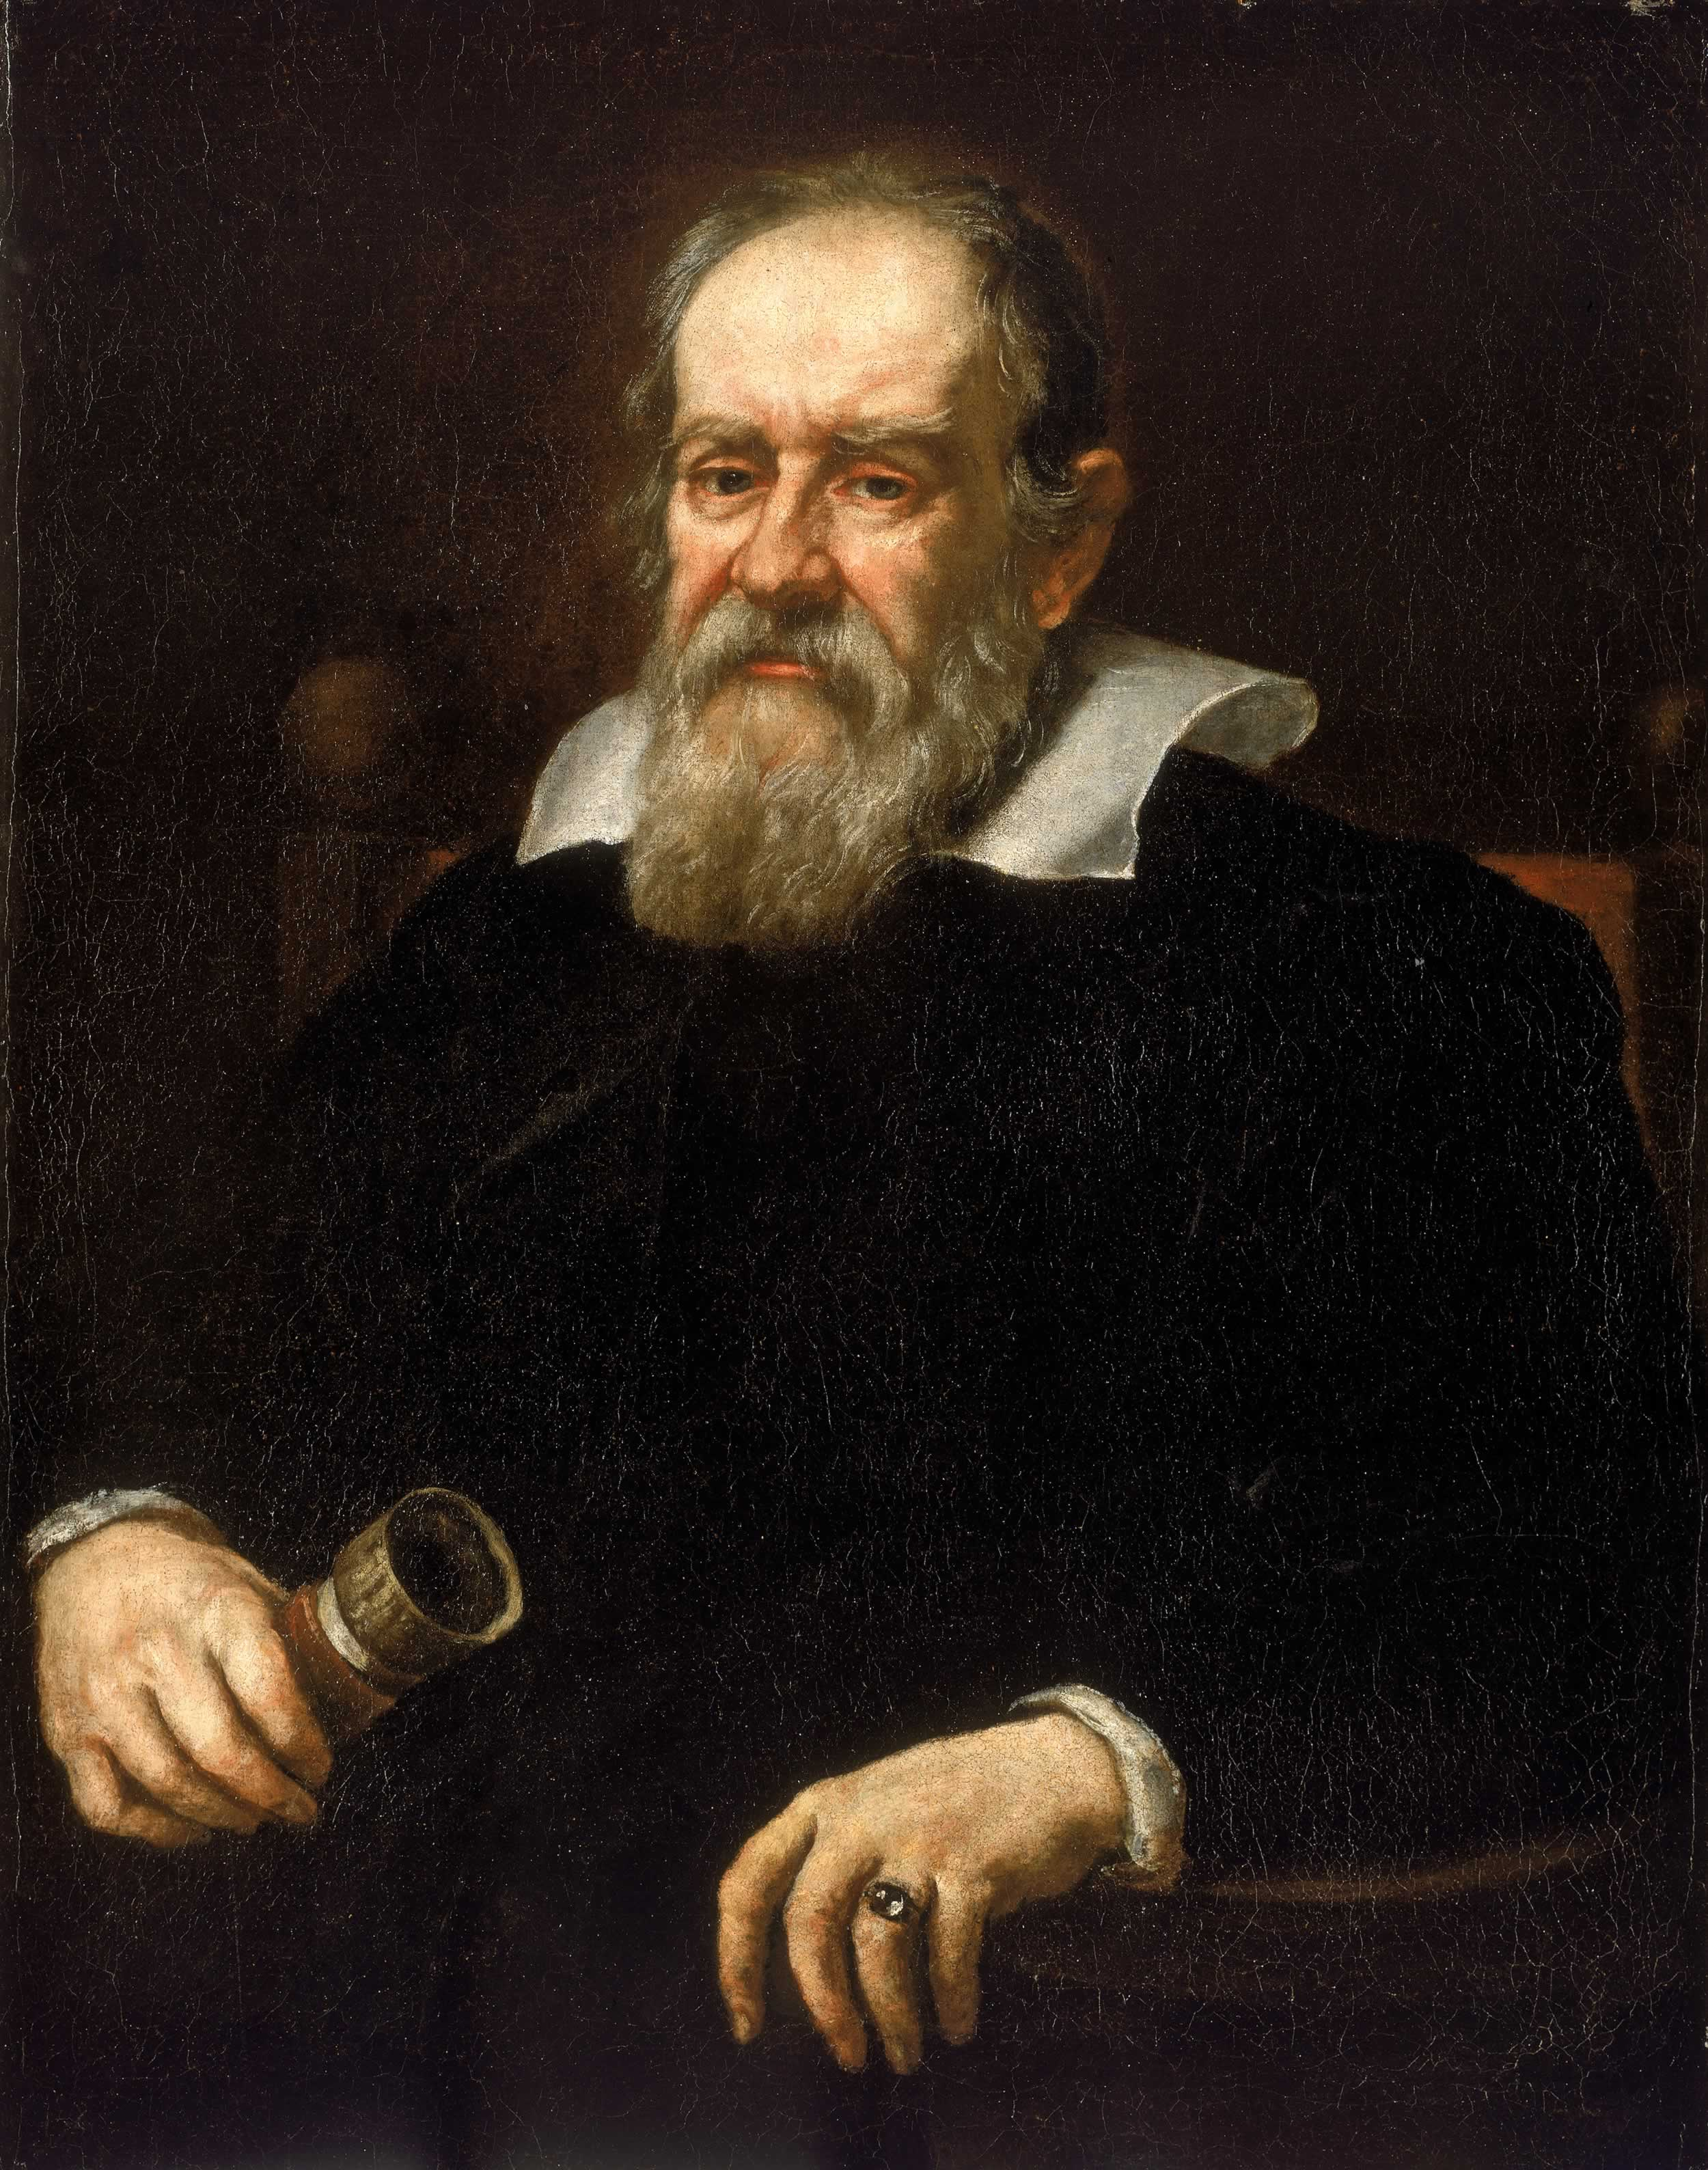
\includegraphics[width=0.4\textwidth]{figures/Galileo.jpg}
    %}{A picture of the Italian polymath Galileio Galilei from Wikimedia commons.}
    \caption{Italian polymath Galileio Galilei, who probably did not drop objects off the leaning tower of Pisa. The image is from \href{https://commons.wikimedia.org/wiki/File:Justus_Sustermans_-_Portrait_of_Galileo_Galilei,_1636.jpg}{Wikimedia Commons}.}
\end{figure}

More precisely Galileo found that (ignoring air resistance) all objects fall at the same rate with their acceleration determined by the gravity acting on the object. This acceleration is known as the \textbf{acceleration due to gravity} $g$ and is approximately constant everywhere on Earth. The value is 
\begin{equation*}
    g=-9.8\text{m/s}^{2}.
\end{equation*}
The minus sign is there because gravity causes objects to accelerate towards the surface of the Earth\footnote{Really they accelerate towards the centre of the Earth but on everyday scales we cannot tell the difference. It also varies with height so if you measure $g$ at the top of a mountain you will get a slightly different answer than if you measure it at sea level, though they will be very close. } and we usually regard upwards as the positive direction.\\

The acceleration due to gravity can be measured by dropping a ball from a known height and timing how long it takes to hit the ground. The second kinematic equation, \cref{eq: Kinematic equation 2} can then be used to solve for the acceleration.  We say that an object only under the influence of gravity is in \textbf{freefall}, as it will keep falling towards the source of gravity until it is stopped by another object, in most cases the surface of the Earth.

\paragraph{Example 3.1:} Consider a coin at rest at the top of a well. If it takes 1.6s to hit the bottom of the well find:
\begin{itemize}
\setlength{\itemsep}{-5pt}
    \item[a)] The depth of the well.
    \item[b)] The speed of the coin just before it hits the bottom of the well.
\end{itemize}

As usual we start by writing down what we know:
\begin{itemize}
\setlength{\itemsep}{-5pt}
    \item $u=0\text{m/s}$ as the coin starts at rest,
    \item $t=1.6\text{s}$,
    \item $a=-9.8\text{m/s}^{2}$ as the coin is falling under gravity.
\end{itemize}

a) We want the depth of the well, this is the displacement of the coin after 1.6s. Use the second kinematic equation and substitute in 
\begin{align*}
    s   &=ut+\frac{1}{2}a t^{2}\\
        &=0 +\frac{1}{2}(-9.8)(1.6)^{2}\\
        &=-12.5\text{m}.
\end{align*}
The minus sign is because this is how far down the coin has fallen and conventionally we think of upwards as the positive direction and downwards as negative.

b) Now we want the final speed of the coin once it has fallen for $1.6$s. Since we know $u,a,$ and $t$, we can use the first kinematic equation to compute this:
\begin{equation*}
    v=u+at =(-9.8)1.6=-15.7\text{m/s}.
\end{equation*}

\section{Vectors}
Now that we have looked at both horizontal and vertical motion it is time to combine them together and study motion in two dimensions. If we wanted to plot displacement against distance in this case we would need to use a three dimensional plot. Usually what is done to visualise the motion is to draw the horizontal and vertical motion separately or to plot horizontal displacement against vertical displacement as in \cref{fig: projectile motion}.\\

\begin{figure}[ht]
    \centering
    %\pdftooltip{
    \ThisAltText{ A plot of projectile motion showing vertical displacement against horizontal displacement.}
    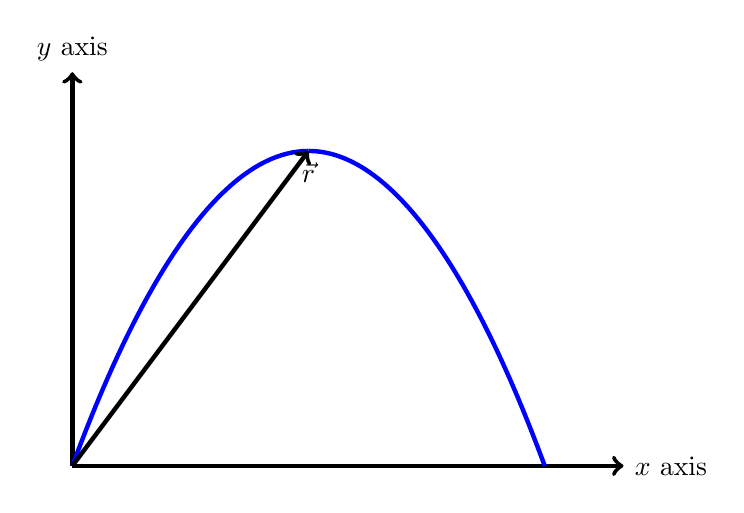
\begin{tikzpicture}
\draw[black, ultra thick,->] (0,0) --(7,0) node[anchor=west]{$x$ axis};
\draw[black, ultra thick,->] (0,0) --(0,5) node[anchor=south]{$y$ axis};
%\draw[step=1cm,gray,very thin] (-2,-2) grid (7,7);
\draw[blue, ultra thick] (3,4) parabola (6,0);
\draw[blue, ultra thick] (3,4) parabola (0,0);
\draw[ultra thick, ->] (0,0) -- (3,4)node[anchor=north]{$\vec{r}$ };
% \filldraw[black] (-4,0) circle (2pt) node[anchor=south]{$x_{1}$ at $t_{1}$};
% \filldraw[black] (4,0) circle (2pt) node[anchor=south]{$x_{2}$ at $t_{2}$};
\end{tikzpicture}
%}{A plot showing projectile motion.}
    \caption{A plot of vertical displacement against horizontal displacement including the vector coordinates of the highest point.}
    \label{fig: projectile motion}
\end{figure}


There are two common, and very closely related, ways to study motion in two, and higher, dimensions:
\begin{itemize}
\setlength{\itemsep}{-5pt}
    \item Study the horizontal and vertical motion separately. This is called working in components and we use the kinematic equations of the previous section but with subscripts on all of the variables to tell us if we are using the horizontal or vertical quantity, e.g. $s_{x}$ for horizontal displacement and $s_{y}$ for vertical displacement or height. 
    \item Work with vectors. 
\end{itemize}

When working in components we write down what we know at the start of a problem separately for the horizontal and vertical cases. e.g. Horizontal motion
    \begin{itemize}
    \setlength{\itemsep}{-5pt}
    \item Initial velocity $u_{x}$.
    \item Final velocity $v_{x}$.
    \item Displacement $s_{x}$.
    \item Acceleration $a_{x}$.
    \item time $t$.
\end{itemize}
Vertical motion
 \begin{itemize}
    \setlength{\itemsep}{-5pt}
    \item Initial velocity $u_{y}$.
    \item Final velocity $v_{y}$.
    \item Displacement $s_{y}$.
    \item Acceleration $a_{y}$.
    \item time $t$.
\end{itemize}
Notice that the time is the same in both cases as we are describing the motion of the same object, just working with the horizontal and vertical pieces separately. If you ever see the words \textbf{neglecting air resistance}, then you can usually assume that $a_{x}=0$ and $a_{y}=g$, that is an object is accelerating vertically due to gravity but is not accelerating horizontally. This is just an approximation but it will serve us fairly well in this module. This is the approach that we will take in the next subsection, and what we will do for most of this course. However, before doing this it is worth having a basic understanding of what is going on with vectors as they will also be important in later weeks when we start discussing forces.\\


\textbf{Vectors} are quantities with both a magnitude and a direction and are usually denoted in either bold or with an arrow on top. For example in \cref{fig: projectile motion} the vector $\vec{r}$ pointing from the origin to the highest point in the objects motion is depicted. The magnitude is the length of the vector and the direction is the angle between the vector and the horizontal axis.\\

\begin{figure}[ht]
    \centering
    \ThisAltText{ A schematic showing how to visualise a vector as a directed line segment.}
    %\pdftooltip{
    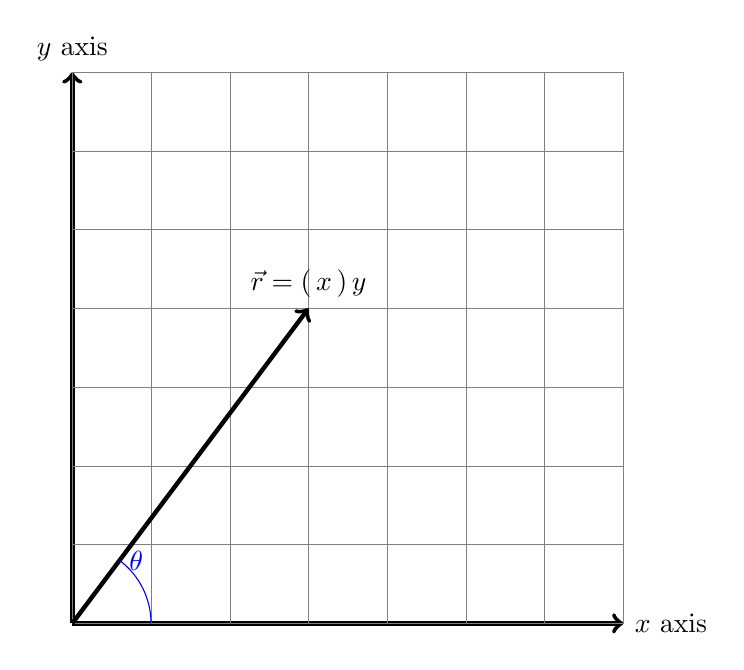
\begin{tikzpicture}
\draw[black, ultra thick,->] (0,0) --(7,0) node[anchor=west]{$x$ axis};
\draw[black, ultra thick,->] (0,0) --(0,7) node[anchor=south]{$y$ axis};
\draw[step=1cm,gray,very thin] (0,0) grid (7,7);
\draw[ultra thick, ->] (0,0) -- (3,4)node[anchor=south]{$\vec{r}=\begin{pmatrix}
    x\\ y
\end{pmatrix}$ };
\draw[blue] (1cm,0cm) arc (0:53.13:1cm)node[ anchor=west]{$\theta$};
% \filldraw[black] (-4,0) circle (2pt) node[anchor=south]{$x_{1}$ at $t_{1}$};
% \filldraw[black] (4,0) circle (2pt) node[anchor=south]{$x_{2}$ at $t_{2}$};
\end{tikzpicture}
%}{A plot showing how to visualise a vector}
    \caption{Two ways to visualise a vector.}
    \label{fig: vectors}
\end{figure}

Another way to think of a vector is as a pair $(x,y)$ of a horizontal position and a vertical position, if we thought of putting a grid on a piece of paper as in \cref{fig: vectors} then the pair $(x,y)$ is one way of specifying a point, while the length of a straight line from the point to the origin and the angle $\theta$ between the line and the horizontal is another way to do this. Vectors can be added, subtracted and multiplied. In fact for addition and subtraction there is a nice geometric picture of what is going on as we take the two vectors, place the start of the second one at the end of the first one and see where it ends, the vector sum is then the straight line pointing from the start of the first vector to the end of the second as in \cref{fig: vector addition}. Similarly when subtracting one vector from another we just add the negative of the second vector to the first as shown in \cref{fig: vector subtraction}.\\

\begin{figure}[ht]
    \centering
   % \pdftooltip{
   \ThisAltText{ A schematic of vector addition where the two vectors are lined up nose to tail and the straight line from the tail of the first to the nose of the second is the vector sum of the two.}
    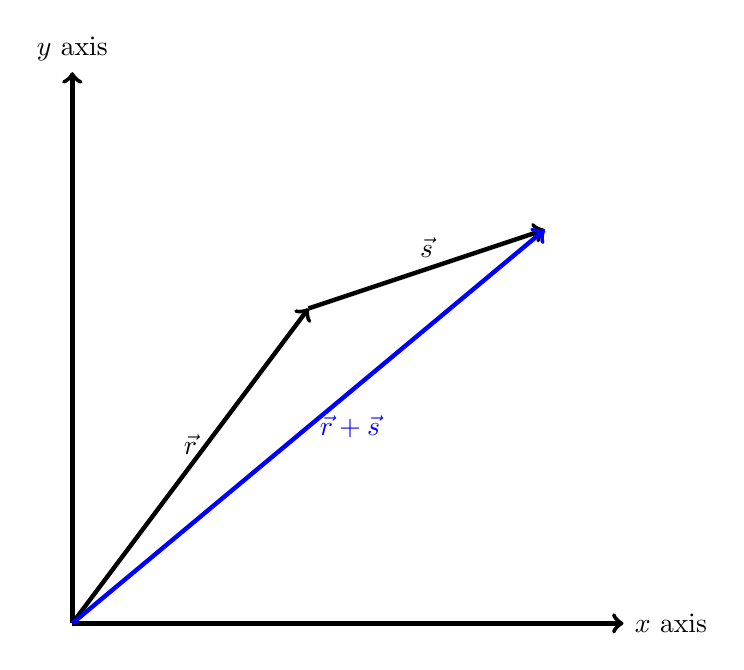
\begin{tikzpicture}
\draw[black, ultra thick,->] (0,0) --(7,0) node[anchor=west]{$x$ axis};
\draw[black, ultra thick,->] (0,0) --(0,7) node[anchor=south]{$y$ axis};
%\draw[step=1cm,gray,very thin] (0,0) grid (7,7);
\draw[ultra thick, ->] (0,0) --node[anchor=south]{$\vec{r}$} (3,4);
\draw[ultra thick, ->] (3,4) --node[anchor=south]{$\vec{s}$} (6,5);
\draw[blue,ultra thick, ->] (0,0) --node[anchor=west]{$\vec{r}+\vec{s}$} (6,5);
% \filldraw[black] (-4,0) circle (2pt) node[anchor=south]{$x_{1}$ at $t_{1}$};
% \filldraw[black] (4,0) circle (2pt) node[anchor=south]{$x_{2}$ at $t_{2}$};
\end{tikzpicture}
%}{vector addition}
    \caption{Vector addition.}
    \label{fig: vector addition}
\end{figure}



\begin{figure}[ht]
    \centering
    %\pdftooltip{
    \ThisAltText{ A schematic of vector subtraction.}
    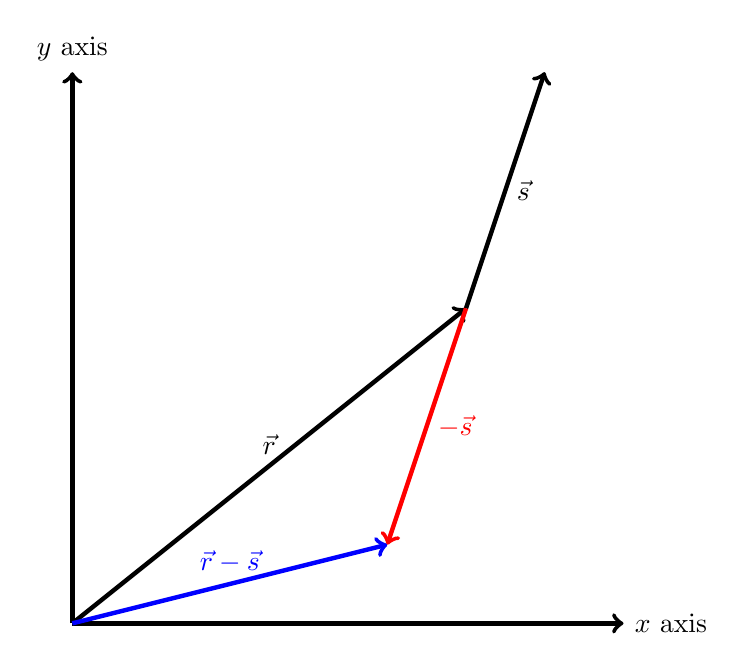
\begin{tikzpicture}
\draw[black, ultra thick,->] (0,0) --(7,0) node[anchor=west]{$x$ axis};
\draw[black, ultra thick,->] (0,0) --(0,7) node[anchor=south]{$y$ axis};
%\draw[step=1cm,gray,very thin] (0,0) grid (7,7);
\draw[ultra thick, ->] (0,0) --node[anchor=south]{$\vec{r}$} (5,4);
\draw[ultra thick, ->] (5,4) --node[anchor=west]{$\vec{s}$} (6,7);
\draw[red, ultra thick, ->] (5,4) --node[anchor=west]{$-\vec{s}$} (4,1);
\draw[blue,ultra thick, ->] (0,0) --node[anchor=south]{$\vec{r}-\vec{s}$} (4,1);
% \filldraw[black] (-4,0) circle (2pt) node[anchor=south]{$x_{1}$ at $t_{1}$};
% \filldraw[black] (4,0) circle (2pt) node[anchor=south]{$x_{2}$ at $t_{2}$};
\end{tikzpicture}
%}{vector subtraction}
    \caption{Vector subtraction.}
    \label{fig: vector subtraction}
\end{figure}

We said that a vector $\vec{r}$ can be expressed in terms of $x$ and $y$ coordinates as 
\begin{equation*}
    \vec{r}=\begin{pmatrix}
        x\\ y
    \end{pmatrix}.
\end{equation*}
The length or modulus of the vector is given by $\vert \vec{r}\vert =\sqrt{x^2 +y^2}$, and the angle is given by 
\begin{equation*}
    \theta=\arctan\left(\frac{y}{x}\right).
\end{equation*}

We need to be careful which quadrant the vector is in as this formula will always return an angle between $-90^{\circ}$ and $90^{\circ}$, we can tell which quadrant the vector is in by drawing it, to get the correct angle we then need to add or subtract $180^{\circ}$ as is appropriate. This means that when $x$ is negative and $y$ is positive then the angle is $180^{\circ}+\arctan\left(\frac{y}{x}\right)$ and when $x$ and $y$ are both negative the angle is $180^{\circ}-\arctan\left(\frac{y}{x}\right)$. Putting this altogether mathematically gives
%\begin{itemize}
%\setlength{\itemsep}{-5pt}
%    \item $\theta =\arctan\left(\frac{y}{x}\right) $ when $x\geq 0$,
%    \item $\theta =180^{\circ}+\arctan\left(\frac{y}{x}\right) $ when$y\geq 0$ and $x<0$,
%    \item $\theta =180^{\circ}-\arctan\left(\frac{y}{x}\right) $ when $x,y <0$.
%\end{itemize}
%Remember that when if we are working in radians then it will be a $\uppi$ that appears instead of $180^{\circ}$.
\begin{equation*}
    \theta =\begin{cases}
        &\arctan\left(\frac{y}{x}\right) \quad \text{When $x\geq 0$,}\\
        &180^{\circ}+\arctan\left(\frac{y}{x}\right)\quad \text{when $y\geq 0$ and $x<0$,}\\
        &180^{\circ}-\arctan\left(\frac{y}{x}\right) \quad \text{When $x,y <0$.}
    \end{cases}
\end{equation*}

Note that when the angle goes beyond $90^{\circ}$ it no longer describes a triangle but the mathematical expressions still make sense. To see why either wait until we discuss circular motion in a later week, or have a look at the mathematical background appendix where a partial explanation of this is given.


\section{Motion in 2D}
We now turn to motion in two dimensions. The most common example of this is \textbf{projectile motion} which is a combination of free fall in the vertical direction and constant speed motion in the horizontal direction.  Projectile motion describes is a good approximation for many things from golf balls and artillery shells, through to thrown stones. We will meet many examples of it in the tutorial problems and in the recommended books. As was mentioned above it is important to start every problem by writing down what we know about the horizontal and vertical motion then identifying what we can compute with that information. This is just like we did with one dimensional motion, but there we did not need to keep track of as many quantities.


\paragraph{Example 3.2:} Consider an arrow fired from the top of a 20 m tower. If the arrow has a horizontal speed of $25 \text{m/s}$, assuming now air resistance find:
\begin{itemize}
\setlength{\itemsep}{-5pt}
    \item[a)] how long the arrow takes to hit the ground,
    \item[b)] the horizontal distance travelled by the arrow\footnote{This is often called the \textbf{range}.}.
\end{itemize}


First write down what we know:

\begin{itemize}
\setlength{\itemsep}{-5pt}
    \item Horizontal:
\begin{itemize}
\setlength{\itemsep}{-5pt}
    \item $t=?$
\item $u_{x}=25\text{m/s}$
\item $v_{x}=u_{x}$, since there is no air resistance we are assuming that $a_{x}=0\text{m/s}^{2}$
\item $s_{x}=?$
\end{itemize}
    \item Vertical:
\begin{itemize}
\setlength{\itemsep}{-5pt}
    \item $t=?$
\item $u_{y}=0\text{m/s}$ as the arrow is fired horizontally
\item $v_{y}=?$
\item $a_{y}=g=-9.8\text{m/s}^{2}$
\item $s_{y}=y=-h=-20m$, this is negative as the arrow will fall $20$m before it hits the ground. 
\end{itemize}
\end{itemize}
a) We want to find the time it takes the arrow to fall $20$ m, this just involves the vertical motion so we can focus on that case and use 
\begin{align*}
s_{y}&=u_{y}t+\frac{1}{2}a_{y}t^{2}\\
&=0+\frac{1}{2}gt^{2},\\
\Rightarrow t&=\sqrt{\frac{2s}{g}}\\
t&=\sqrt{\frac{2\times 20}{9.8}}=2.02 \text{s}.
\end{align*}
If you prefer to rearrange the equation after you have substituted in the numbers then that is ok, just be careful that you do not introduce any rounding errors. Also, note that since the time is always positive we can ignore the negative square root when solving for $t$, if we were solving for a position then we would need to include both\footnote{In the future we will meet examples where $u\neq 0$ and then we have to solve a quadratic equation for $t$ which has two roots, often $t=0$ and another positive value of $t$. }.\\

b) Now we want the horizontal distance travelled and since we know the time that the arrow is in the air for, from part a), and we know that $u_{x}$ is constant, we can use 
\begin{equation*}
s_{x}=u_{x}t=25\times 2.02=50.5\text{m}.
\end{equation*}
So the arrow travel $50.5$ m before it hits the ground.

Often we will be given the velocity in a given direction, and an angle specifying that direction, rather than being given the horizontal and vertical velocities separately. This means that we need to be able to use trigonometry to extract $v_{x}$ and $v_{y}$ from what we are given. See \cref{fig: velocity components} for an example of what this looks like. 
\begin{figure}[ht]
    \centering
    %\pdftooltip{
    \ThisAltText{ A velocity vector decomposed into its horizontal and vertical components.}
    \begin{tikzpicture}[scale=2]
  \coordinate [label=left:$\theta$] (C) at (-1.5cm,-1.cm);
  \coordinate (A) at (1.5cm,-1.0cm);
  \coordinate (B) at (1.5cm,1.0cm);
  \draw (C) -- node[above] {$v$} (B) -- node[right] {$v_{y}$} (A) -- node[below] {$v_{x}$} (C);
  \draw (1.25cm,-1.0cm) rectangle (1.5cm,-0.75cm);
  \tkzMarkAngle[size=1cm,color=blue](A,C,B)
 % \tkzMarkAngle[size=1cm,color=blue](C,B,A)
\end{tikzpicture}
%}{A velocity vector and how it is decomposed into horizontal and vertical components.}
    \caption{A velocity vector and how it is decomposed into horizontal and vertical components.}
    \label{fig: velocity components}
\end{figure}

The key point is that using trigonometry we have that
\begin{align*}
v_{x}&=v\cos\theta,\\
v_{y}&=v\sin\theta.
\end{align*}
There will be lots of opportunity to practice these sorts of problems as well. If you need a reminder about how to use trigonometry then have a look at the appendix on mathematical background or check out some of the links to further reading.

\paragraph{Example 3.3:} Consider an arrow fired at a velocity of $48\text{m/s}$ at an agle of $30^{\circ}$ above the horizontal from a height of $1.5$ m above flat ground. Calculate the maximum height that the arrow reaches, e.g. the peak of the parabola.\\

First we are being asked to find the maximum height, is there anything special about where an object reaches its maximum height? Yes, before the maximum it is going up while after the maximum it is going down, this means that the vertical velocity has changed direction, and it can only do this if it has gone to zero at the maximum height. The maximum height is thus the point where the vertical velocity vanishes, $v_{y}=0$ m/s. In this case we just need to solve a one dimensional problem using the vertical motion. 

We know that:
\begin{itemize}
\setlength{\itemsep}{-5pt}
    \item $t=?$
\item $u_{y}=48\sin\left(30^{\circ}\right)=24\text{m/s}$
\item $v_{y}=0$m/s
\item $a_{y}=g=-9.8\text{m/s}^{2}$
\item $s_{y}=?$
\end{itemize}

Now use
\begin{align*}
v_{y}^{2}&=u_{y}^{2}+2a_{y}s_{y},\\
\Rightarrow s_{y}&=\frac{v_{y}^{2}-u_{y}^{2}}{2a_{y}}\\
&=\frac{0-(24)^{2}}{-2\times 9.8}\\
&=29.3\text{m}
\end{align*}

This is the height the arrow travels from above its starting point, however it starts at $1.5$ m above the ground so attains a maximum height above the ground of $30.8$ m. 

An alternative way to solve this problem would be to use the first kinematic equation, \cref{eq: Kinematic equation 1}, to find $t$ and then substitute this into the second kinematic equation, \cref{eq: Kinematic equation 2}, then solving for $s_{y}$.\\



\paragraph{Example 3.4:} A Batter hits a baseball so that it leaves the bat at a speed of $u=37.0\text{m/s}$ at an angle of $\theta=53.1^{\circ}$. Find:
\begin{itemize}
\setlength{\itemsep}{-5pt}
    \item[a)] The horizontal and vertical components of the velocity at $t=0$ s.
    \item[b)] The position of the ball and its speed after 2s.
    \item[c)] The maximum height reached by the ball and how long it takes to reach this height.
    \item[d)] The range of the ball before it hits the ground.
\end{itemize}
This is a complicated question with several stages, if you can solve this problem then you can solve any of the projectile motion questions that you will come across on the tutorial sheet or on the exam. This brings together everything that we have seen so far.

a) Use trigonometry to calculate the components as
\begin{align*}
u_{x}&=u\cos\theta =37\times \cos53.1^{\circ}=22.2 \text{m/s},\\
u_{y}&=u\sin\theta =37\times \sin53.1^{\circ}=29.6 \text{m/s}.
\end{align*}

b) Let's list what we know and what we do not know:
\begin{itemize}
\setlength{\itemsep}{-5pt}
    \item Horizontal:
\begin{itemize}
\setlength{\itemsep}{-5pt}
    \item $t=2$s
\item $v_{x}=u_{x}=22.2\text{m/s}$ 
\item $s_{x}=?$
\end{itemize}
    \item Vertical:
\begin{itemize}
\setlength{\itemsep}{-5pt}
    \item $t=2$s
\item $u_{y}=29.6\text{m/s}$ as the arrow is fired horizontally
\item $v_{y}=?$
\item $a_{y}=g=-9.8\text{m/s}^{2}$
\item $s_{y}=?$.
\end{itemize}
\end{itemize}
We want both $s_{x}$ and $s_{y}$ so first calculate horizontal then vertical position using kinematic equations:
\begin{align*}
s_{x}&=u_{x}t=22.2\times 2=44.4\text{m},\\
s_{y}&=u_{y}t+\frac{1}{2}a_{y}t^{2}=29.6\times 2+\frac{1}{2}(-9.8)\times 4=39.6\text{m}.
\end{align*}
For the speed we need $v_{y}$ and then can use that the speed is calculated from the velocity as $\text{speed}=\sqrt{v^{2}_{x}+v^{2}_{y}}$. Thus:
\begin{align*}
v_{y}&=u_{y}+a_{y}t=29.6-9.8\times 2=10\text{m/s},\\
\text{speed}&=\sqrt{v^{2}_{x}+v^{2}_{y}}=24.3\text{m/s}.
\end{align*}

c) Now we want to find the maximum height reached by the ball. Recall that $v_{y}=0$ at the maximum height, we can either compute the time using $v_{y}=u_{y}+a_{y}t$ then use this to compute $s_{y}$ through $s_{y}=u_{y}t+\frac{1}{2}a_{y}t^{2}$ or we can use the third kinematic equation, \cref{eq: Kinematic equation 3} to solve for $s_{y}$ directly as
\begin{align*}
v^{2}_{y}&=u^{2}_{y}+2a_{y}s_{y},\\
\Rightarrow s_{y}&=\frac{v^{2}_{y}-u^{2}_{y}}{2a_{y}}\\
s_{y}&=\frac{(29.6)^{2}}{9.8\times 2}= 44.7\text{m}.
\end{align*}

d) Finally, we want to find the range of the ball, that is how far it travels horizontally before hitting the ground. We do this in two steps: 1) find the time it takes the ball to hit the ground by studying the vertical motion, 2) use $t$ and the horizontal motion to find the range.

1) The ground is at $s_{y}=0$ so for the vertical motion we know that:
\begin{itemize}
\setlength{\itemsep}{-5pt}
    \item $t=?$
\item $u_{y}=29.6\text{m/s}$ as the arrow is fired horizontally
\item $v_{y}=?$
\item $a_{y}=g=-9.8\text{m/s}^{2}$
\item $s_{y}=0$m.
\end{itemize}
To find for $t$ we use the second kinematic equation to get a quadratic equation for $t$ that we can then solve:
\begin{align*}
s_{y}&=u_{y}t+\frac{1}{2}a_{y}t^{2}\\
0&=t\left(u_{y}+\frac{1}{2}a_{y}t\right),
\end{align*}
so $t=0$ or $t=-2u_{y}/a_{y}$. Note that getting two values of $t$ makes sense as the ball is at ground level at two times, first when it is hit initially and then when it returns to the ground.  Plugging in the numbers gives that
\begin{equation*}
t=-\frac{2u_{y}}{a_{y}}=\frac{2\times 29.6}{9.8}=6.04\text{s}
\end{equation*}

2) Now that we have $t$ we can solve for $s_{x}$ as
\begin{equation*}
s_{x}=u_{x}t=22.2\times 6.04 =134\text{m}.
\end{equation*}
